\section{Test}

\subsection{Multitrådet sum}
Implementationen er testet ved først at køre \texttt{sum} på en enkelt tråd, med et antal iterationer, der kan beregnes i hånden.
Herefter kørtes implementationen på flere kerner, for at se, at resultatet var det samme. 
Programmet blev kørt på flere computere, for at teste hastighedsforskellen med flere eller færre kerner. 
Nedenstående graf viser resultaterne ved kørsel på en 4-kernet maskine. Det er værd at lægge mærke til, at der ikke er nogen hastighedsforøgelse efter at alle maskinens kerner er i brug. 

\begin{figure}[h!]
\center
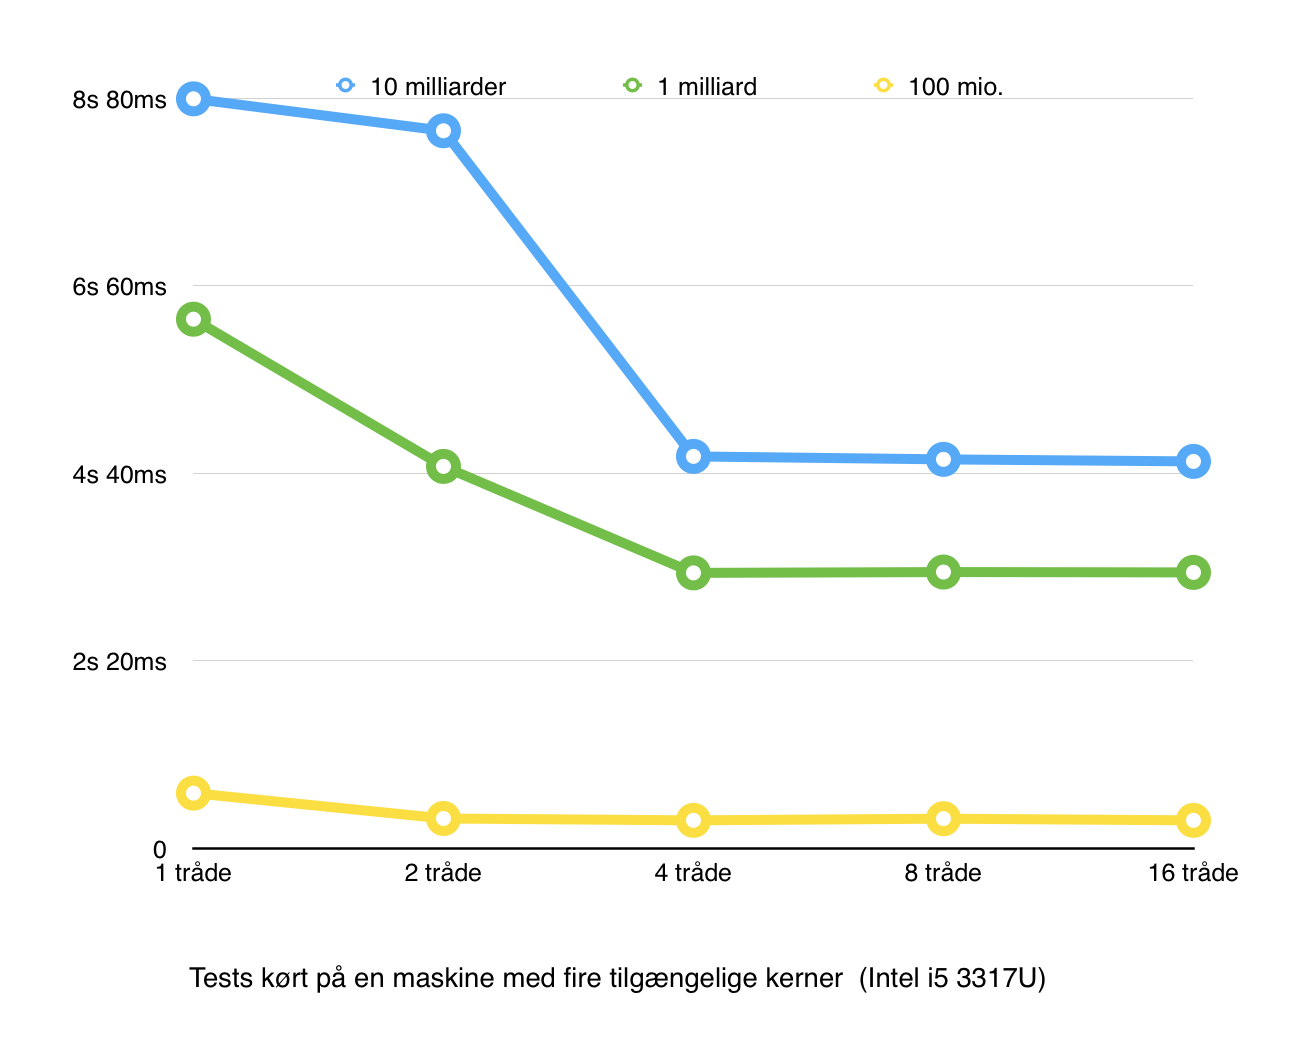
\includegraphics[width=\linewidth]{../figures/graph.png}
\end{figure}

\subsection{Multitrådet FIFO kædet liste}
For at teste at list.c ikke introducere race conditions er \texttt{fifotest.c} implementeret. Programmet tager to argumenter, antal iterationer programmet skal køre og antal tråde programmet skal sætte til at køre iterationerne. Hver tråd danner to unikke elementer og tilføjer dem til den globale liste, hvorefter tråden fjerner dem igen. Den fjernede nodes \texttt{elm} member gemmes herefter i et globalt to-dimensionelt char array kaldet \texttt{results}. Dette gøres ligeså mange gange som værdien af programmets første parameter. \\

Efter alle trådene er kørt tjekkes det at der ikke eksisterer to a samme char array i \texttt{result}. Derefter tjekkes det også at den globale listes \texttt{len} member er 0. Denne test tjekker altså om et eller flere elementer er blevet fjernet fra listen to eller flere gange og derved om to eller flere tråde har fået adgang til den samme ressource på samme tidspunkt - en race condition.

\texttt{fifotest.c} er kørt med argumenterne 10000 og 16. Hvis linjerne 26, 35, 41, 49 og 57 er udkommenteret i \texttt{list.c} er det lykkedes at fremprovokere en race condition. Uden at have udkommeteret de nævnte linjer har det ikke været muligt at få en racecondition.

\subsection{Producer-Consumer med bounded buffer}

\subsection{Banker's algorithm til håndtering af deadlock}
